\chapter{Other Factors}

\section{Evidence of Other factors}

In the following example, the same anchor set is used in four different random networks.  Figures~\ref{fig:AS6good1} and \ref{fig:AS6good2} show two non-outlier cases.  Figures~\ref{fig:AS6NetworkDiff7} and \ref{fig:AS6NetworkDiff10} plot a line between the real and calculated location of each node, giving a visual representation of the error.  That same data is interpolated into a contour plot in Figures~\ref{fig:AS6NetworkContour7} and \ref{fig:AS6NetworkContour7}.

Not surprisingly, the mean error for each network, despite have the same anchor set, is different.  What is surprising in the degree to which they are different: 37\%.  While it is clear that anchor placement does play a role, there are significant other factors affecting the localization error.

\begin{figure}
  \centering
	\subfloat[Network A]{\label{fig:AS6NetworkDiff7}
		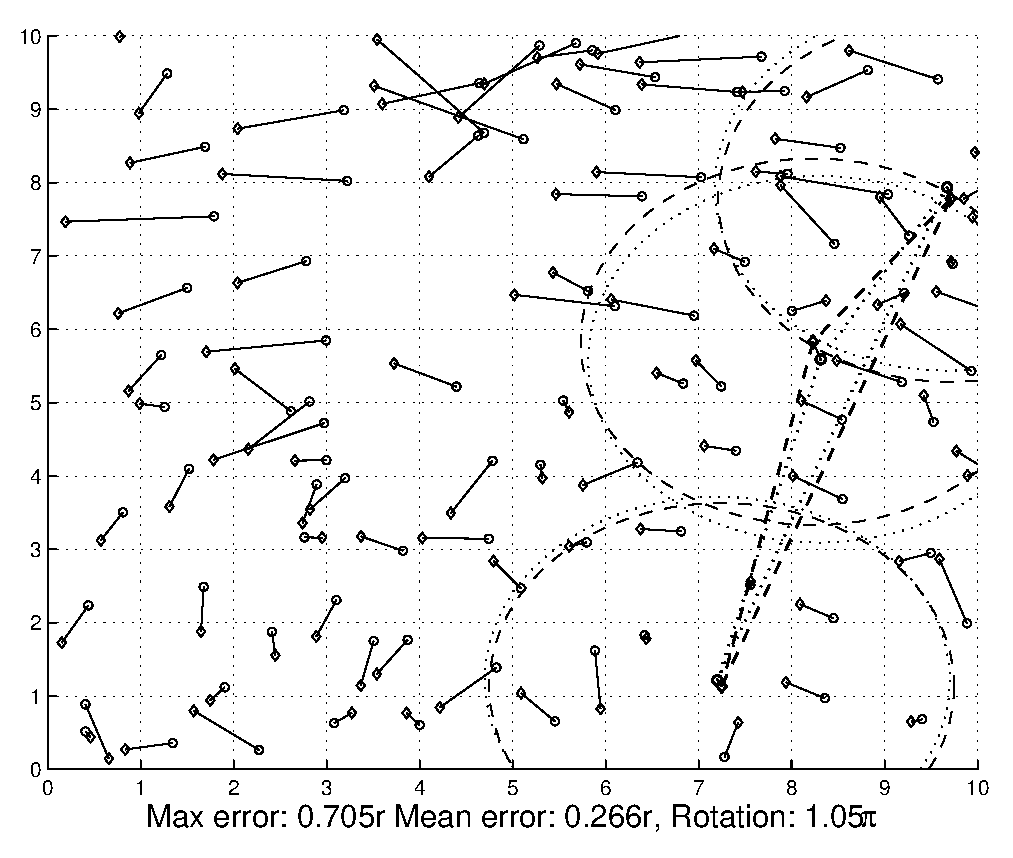
\includegraphics[width=\figurewidth\textwidth]{outliers/AS6/AS6NetworkDiff7}}
\\
	\subfloat[Network A]{\label{fig:AS6NetworkContour7}	
		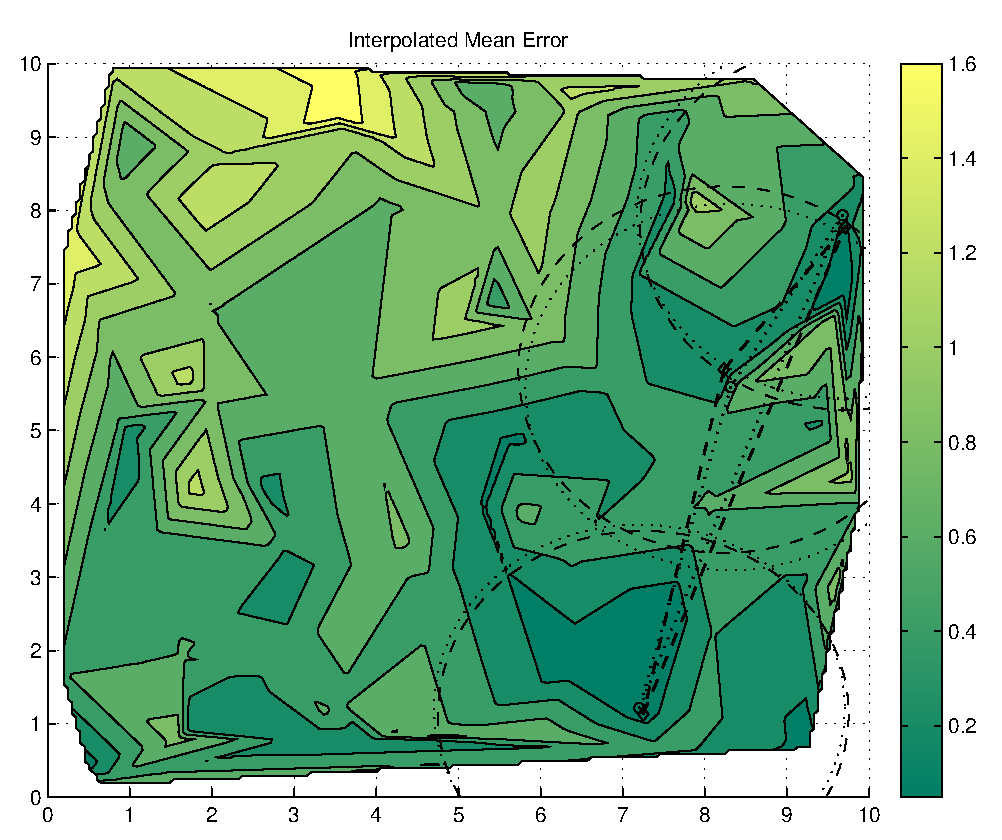
\includegraphics[width=\figurewidth\textwidth]{outliers/AS6/AS6NetworkContour7}}
	\label{fig:AS6good1}		
\end{figure}
\begin{figure}
  \centering
	\subfloat[Network B]{\label{fig:AS6NetworkDiff10}
		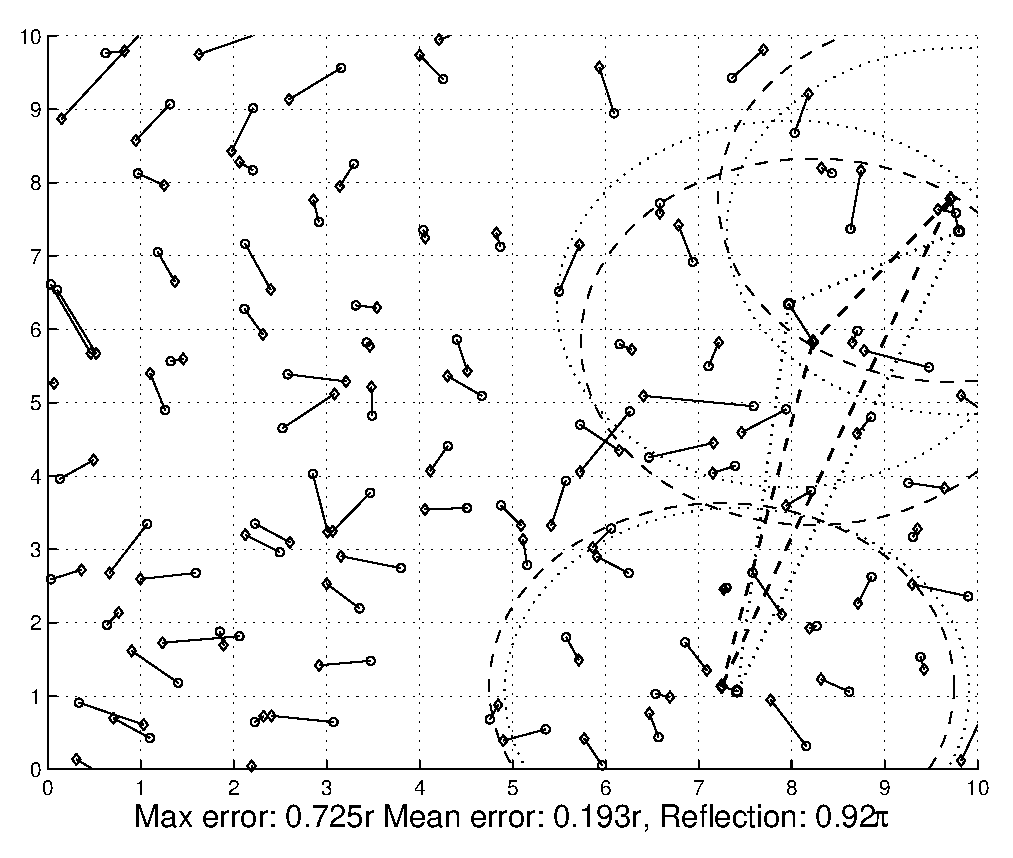
\includegraphics[width=\figurewidth\textwidth]{outliers/AS6/AS6NetworkDiff10}}
\\
	\subfloat[Network B]{\label{fig:AS6NetworkContour10}	
		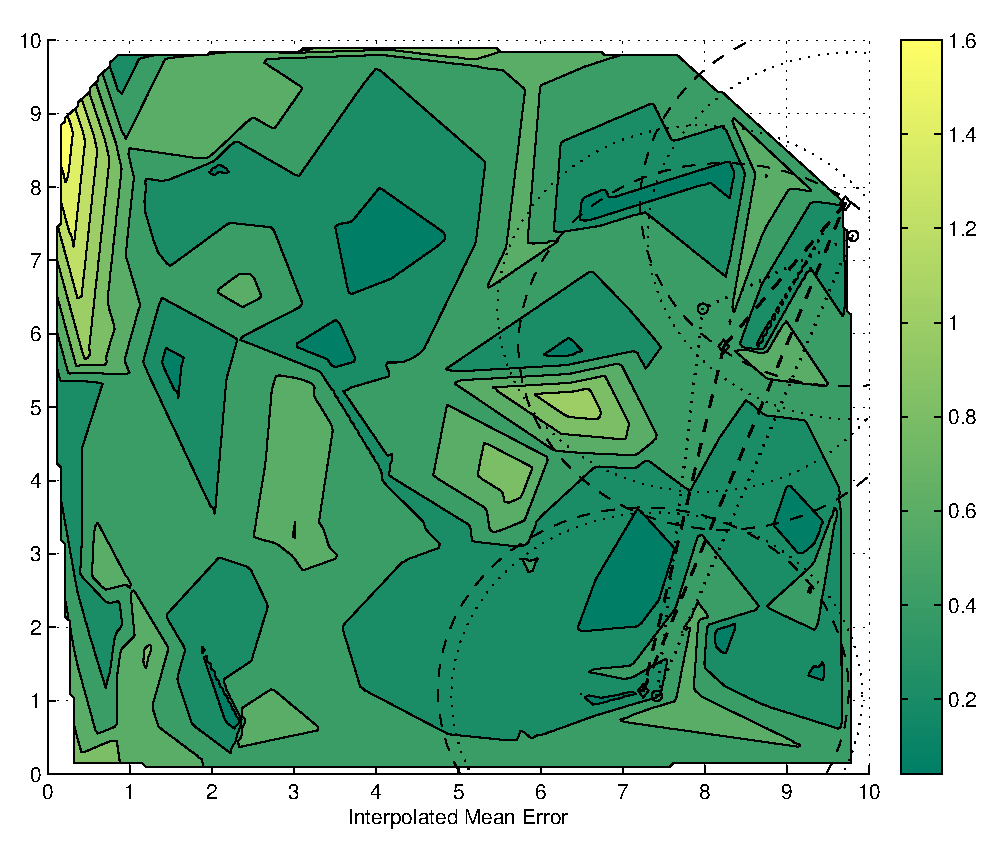
\includegraphics[width=\figurewidth\textwidth]{outliers/AS6/AS6NetworkContour10}}
	\caption{Another different network with the same anchor set}
	\label{fig:AS6good2}
\end{figure}

Further, Figures~\ref{fig:AS6bad1} and \ref{fig:AS6bad2} show two more random networks, using the same anchor set as above.  As seen in the Chapter~\ref{chap:outliers}, some short anchor node triangles can cause extremely poor localization.  In this case, we see that even the same anchor set does not necessarily mean that the resulting localization results will so poor.  

\begin{figure}
  \centering
	\subfloat[Network C]{\label{fig:AS6NetworkDiff9}
		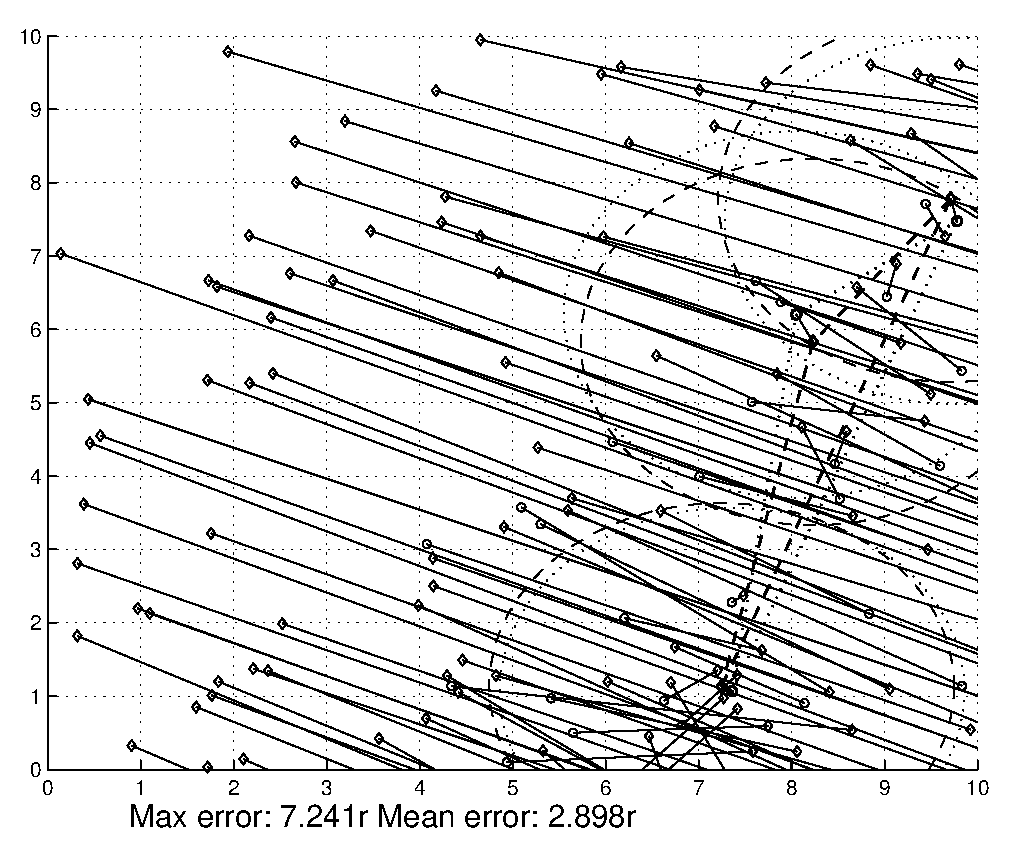
\includegraphics[width=\figurewidth\textwidth]{outliers/AS6/AS6NetworkDiff9}}
\\
	\subfloat[Network C]{\label{fig:AS6NetworkContour9}	
		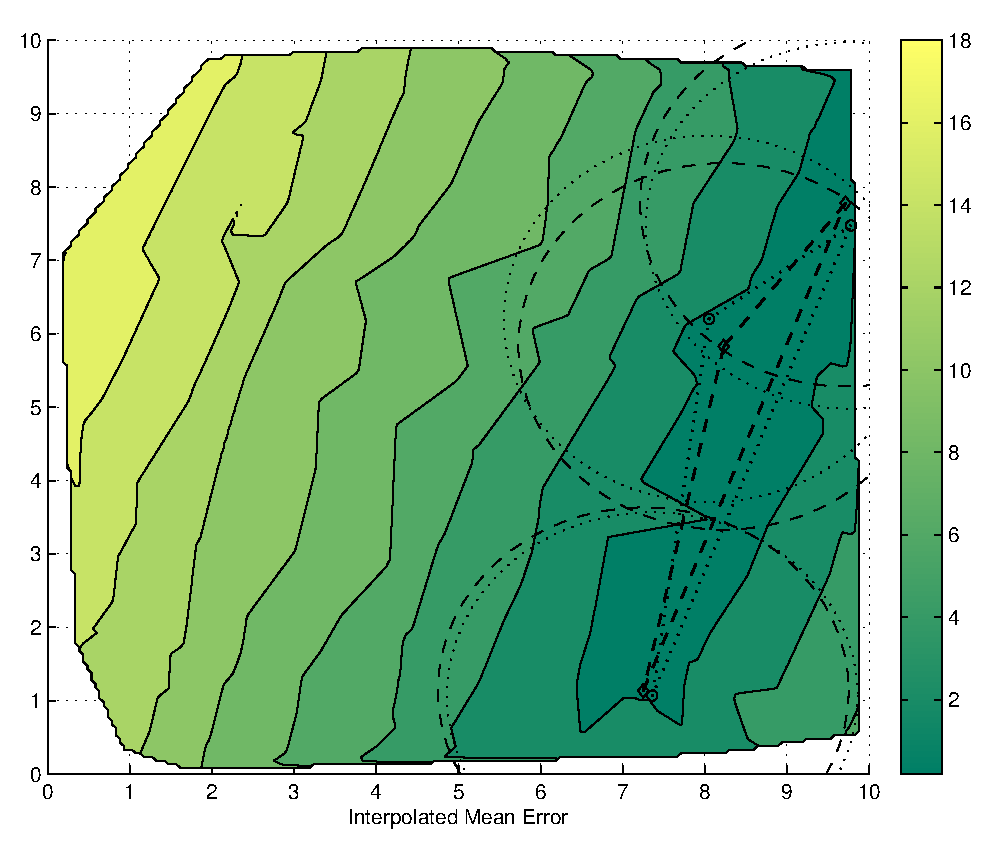
\includegraphics[width=\figurewidth\textwidth]{outliers/AS6/AS6NetworkContour9}}
    \caption{Another different network with the same anchor set}	
	\label{fig:AS6bad1}
\end{figure}
\begin{figure}
  \centering
	\subfloat[Network D]{\label{AS6NetworkDiff8}
		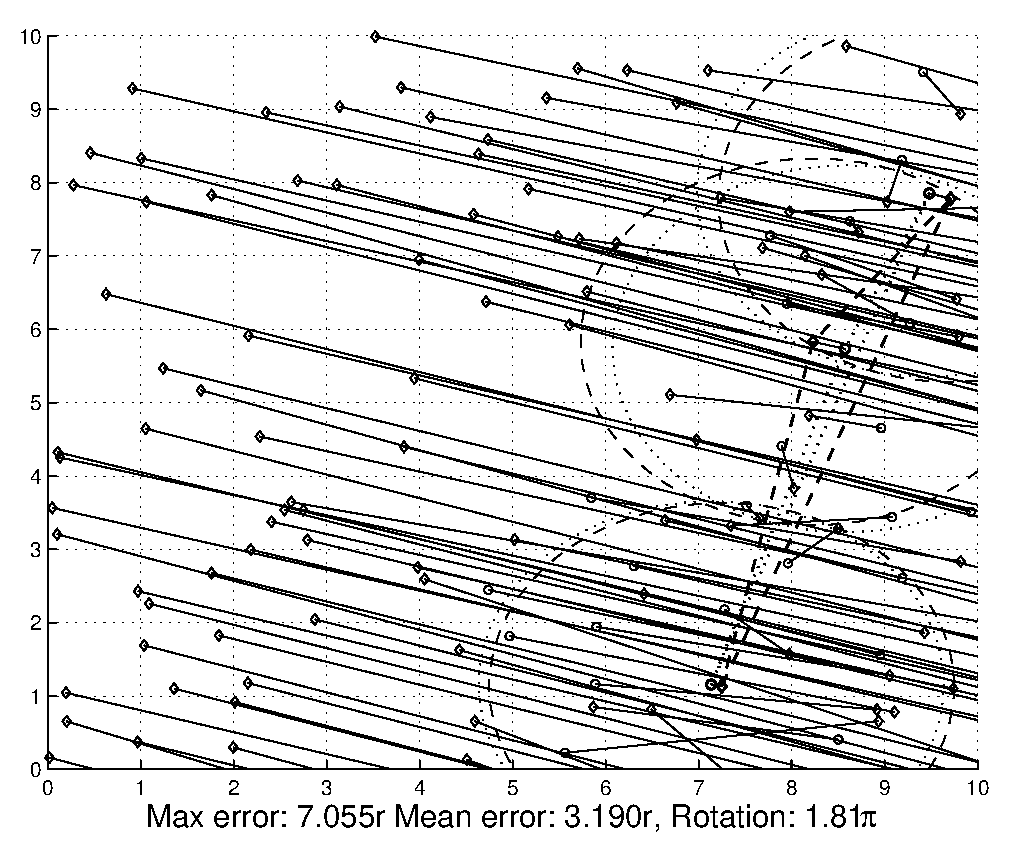
\includegraphics[width=\figurewidth\textwidth]{outliers/AS6/AS6NetworkDiff8}}	
	\subfloat[Network D]{\label{fig:AS6NetworkContour8}	
		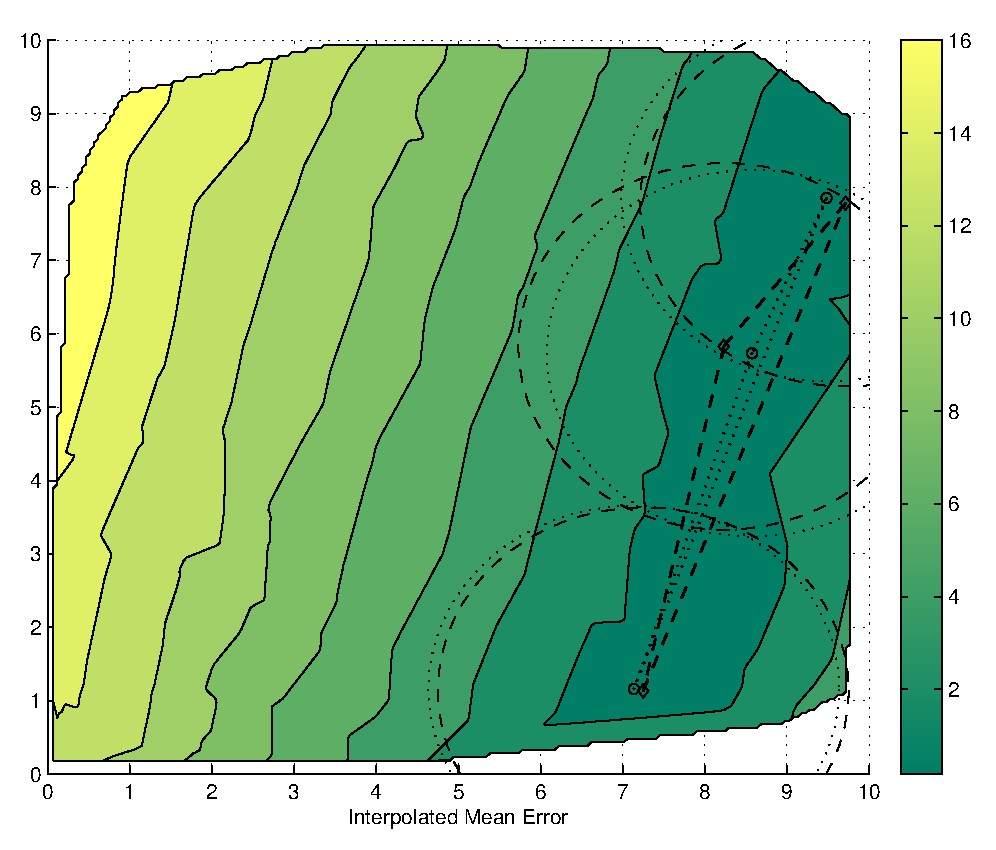
\includegraphics[width=\figurewidth\textwidth]{outliers/AS6/AS6NetworkContour8}}
	\caption{Another different network with the same anchor set}	
	\label{fig:AS6bad2}
\end{figure}
